% Beamer Presentation
% LaTeX Template
% Version 1.0 (10/11/12)
%
% This template has been downloaded from:
% http://www.LaTeXTemplates.com
%
% License:
% CC BY-NC-SA 3.0 (http://creativecommons.org/licenses/by-nc-sa/3.0/)
%
%%%%%%%%%%%%%%%%%%%%%%%%%%%%%%%%%%%%%%%%%

%----------------------------------------------------------------------------------------
%	PACKAGES AND THEMES
%----------------------------------------------------------------------------------------

\documentclass{beamer}

\mode<presentation> {

% The Beamer class comes with a number of default slide themes
% which change the colors and layouts of slides. Below this is a list
% of all the themes, uncomment each in turn to see what they look like.

%\usetheme{default}
%\usetheme{AnnArbor}
%\usetheme{Antibes}
%\usetheme{Bergen}
%\usetheme{Berkeley}
%\usetheme{Berlin}
%\usetheme{Boadilla}
%\usetheme{CambridgeUS}
%\usetheme{Copenhagen}
%\usetheme{Darmstadt}
%\usetheme{Dresden}
%\usetheme{Frankfurt}
%\usetheme{Goettingen}
\usetheme{Hannover}
%\usetheme{Ilmenau}
%\usetheme{JuanLesPins}
%\usetheme{Luebeck}
%\usetheme{Madrid}
%\usetheme{Malmoe}
%\usetheme{Marburg}
%\usetheme{Montpellier}
%\usetheme{PaloAlto}
%\usetheme{Pittsburgh}
%\usetheme{Rochester}
%\usetheme{Singapore}
%\usetheme{Szeged}
%\usetheme{Warsaw}

% As well as themes, the Beamer class has a number of color themes
% for any slide theme. Uncomment each of these in turn to see how it
% changes the colors of your current slide theme.

%\usecolortheme{albatross}
%\usecolortheme{beaver}
%\usecolortheme{beetle}
%\usecolortheme{crane}
%\usecolortheme{dolphin}
%\usecolortheme{dove}
%\usecolortheme{fly}
%\usecolortheme{lily}
%\usecolortheme{orchid}
%\usecolortheme{rose}
%\usecolortheme{seagull}
%\usecolortheme{seahorse}
%\usecolortheme{whale}
%\usecolortheme{wolverine}

%\setbeamertemplate{footline} % To remove the footer line in all slides uncomment this line
%\setbeamertemplate{footline}[page number] % To replace the footer line in all slides with a simple slide count uncomment this line

%\setbeamertemplate{navigation symbols}{} % To remove the navigation symbols from the bottom of all slides uncomment this line
}

\usepackage{graphicx} % Allows including images
\usepackage{booktabs} % Allows the use of \toprule, \midrule and \bottomrule in tables
\usepackage[brazil]{babel}
\usepackage[utf8]{inputenc}
\usepackage{graphicx}
%\usepackage{epstopdf}

\graphicspath{ {./imagens/} }

\newcounter{saveenumi}
\newcommand{\seti}{\setcounter{saveenumi}{\value{enumi}}}
\newcommand{\conti}{\setcounter{enumi}{\value{saveenumi}}}

%----------------------------------------------------------------------------------------
%	TITLE PAGE
%----------------------------------------------------------------------------------------

\title[TCC]{Implementação e análise de performance do algoritmo Pollard's Rho para ataque à segurança de curvas elípticas} % The short title appears at the bottom of every slide, the full title is only on the title page

\author[Rodrigo Gonçalves \and Carlos Teixeira]{Rodrigo Gonçalves \and Carlos Teixeira\\ \and \textbf{Orientador} Luiz Laranjeira\\ \and \textbf{Coorientador} Edson Alves}

\institute[UnB-FGA] % Your institution as it will appear on the bottom of every slide, may be shorthand to save space
{
Universidade de Brasília - Campus Gama - FGA\\ % Your institution for the title page
\medskip
%\textit{rodrigosg2000@gmail.com \and carlostjunior517@gmail.com} % Your email address
}
\date{\today} % Date, can be changed to a custom date

%---------------------------------------------------------------------------------------
%         DOCUMENT
%---------------------------------------------------------------------------------------

\begin{document}

\begin{frame}
\titlepage % Print the title page as the first slide
\end{frame}

\begin{frame}
\frametitle{Agenda} % Table of contents slide, comment this block out to remove it
\tableofcontents % Throughout your presentation, if you choose to use \section{} and \subsection{} commands, these will automatically be printed on this slide as an overview of your presentation


\end{frame}

%
% INTRODUÇÂO
%

%-----------------------------------------------------------------------------------------------
\section{Introdução}
\begin{frame}

Curvas elípticas são estruturas definidas por equações cúbicas

\begin{figure}
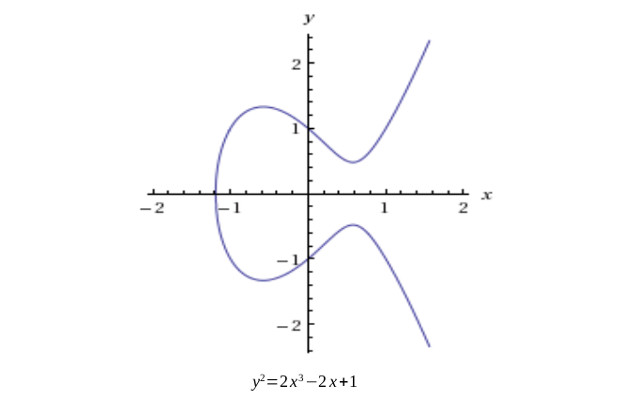
\includegraphics[scale = 0.3]{curva_eliptica}
\end{figure}

\end{frame}
%-----------------------------------------------------------------------------------------------

\begin{frame}
\frametitle{Objetivos}
\begin{itemize}
\item Estudar os conceitos matemáticos mais importantes sobre curvas elípticas e sua aplicação na criptografia
\item Implementar o algoritmo Pollard's rho e suas variações
\item Analisar os desempenhos práticos dos algoritmos implementados
\end{itemize}
\end{frame}
%-----------------------------------------------------------------------------------------------

%
% CURVAS ELIPTICAS
%

%-----------------------------------------------------------------------------------------------
\section{Curvas Elípticas}
\begin{frame}
\begin{itemize}
\item Uma curva elíptica é o conjunto de soluções de uma equação cúbica definida sobre um corpo $\mathbb{F}$
\item Pode ser representada pela equação de Weierstrass
$$ y^2 + axy + by = x^3 + cx^2 + dx + e$$
\item Com frequência, no estudo de criptografia, costuma-se usar a equação reduzida de Weierstrass
$$ y^2 = x^3 + ax + b $$
\item No entanto é imprescindível que seja satisfeita a condição
$$ 4a^3 + 27b^2 \neq 0$$
\end{itemize}
\end{frame}
%-----------------------------------------------------------------------------------------------

%
% PROBLEMA DO LOGARITMO DISCRETO
%

%-----------------------------------------------------------------------------------------------
\section{Problema do logaritmo discreto}
\begin{frame}
\begin{columns}[c]
\column{.45\textwidth}
\begin{itemize}
\item Sejam dois pontos $P$ e $Q$ pertencentes à uma curva, encontrar o valor de $x$ tal que $xP = Q$
\item Computacionalmente caro
\item Um valor muito alto de k inviabiliza análise de força bruta
\item Existem alguns algoritmos que tentam resolver este problema
\end{itemize}

\column{.5\textwidth}
\begin{figure}
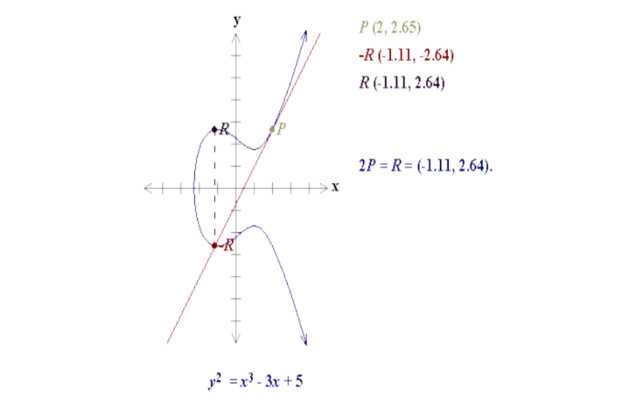
\includegraphics[scale=0.3]{multiplicacao_ponto}
\end{figure}
\end{columns}
\end{frame}
%-----------------------------------------------------------------------------------------------

%
% CICLO DE FLOYD
%

%-----------------------------------------------------------------------------------------------
\section{Ciclo de Floyd}
\begin{frame}

\end{frame}
%-----------------------------------------------------------------------------------------------

%
% POLLARD RHO ORIGINAL
%

%-----------------------------------------------------------------------------------------------
\section{Pollard's Rho original}
\begin{frame}
Encontrar pares distintos $(a,b)$ e $(a',b')$ tais que
$$aP + bQ = a'P + b'Q$$

Pelo problema do logaritmo discreto, $Q = lP$, logo, é possível obter $l$ através da equação
$$l = (a - a')(b' - b)^{-1} \mbox{mod }n$$
\end{frame}
%------------------------------------------------------------------------------------------------
\begin{frame}
  \begin{enumerate}
    \item Usar uma função para particionar o conjunto de pontos $E(\mathbb{F}_p)$ em 3 subconjuntos $S_1, S_2, S_3$, com tamanhos aproximados.
    \item Definir uma função de passo aleatório $f$ como função de iteração
    $$
      R_{i+1}=\left\{\begin{array}{rc}
      Q + R_i,&\mbox{se}\quad R_i \in S_1,\\
      2R_i,&\mbox{se}\quad R_i \in S_2,\\
      P + R_i,&\mbox{se}\quad R_i \in S_3,\\
      \end{array}\right.
    $$ 
    \seti
  \end{enumerate}
\end{frame}
%------------------------------------------------------------------------------------------------
\begin{frame}
  \begin{enumerate}
    \conti
    \item Seja $R_i = a_iP + b_iQ$ fazer as funções
      $$
        a_{i+1}=\left\{\begin{array}{rc}
        a_i,&\mbox{se}\quad R_i \in S_1,\\
        2a_i \mbox{ mod }n,&\mbox{se}\quad R_i \in S_2,\\
        a_i + 1,&\mbox{se}\quad R_i \in S_3,\\
        \end{array}\right.
      $$
      $$
        b_{i+1}=\left\{\begin{array}{rc}
        b_i + 1,&\mbox{se}\quad R_i \in S_1,\\
        2b_i \mbox{ mod }n,&\mbox{se}\quad R_i \in S_2,\\
        b_i,&\mbox{se}\quad R_i \in S_3,\\
        \end{array}\right.
      $$
    \item Usar como ponto de partida $R_0 = P, a_0 = 1, b_0 = 0$, e gerar os pares $(R_i, R_{2i})$ até encontrar uma colisão
      $$ R_i = R_{2i} $$
    \conti
  \end{enumerate}
\end{frame}
%--------------------------------------------------------------------------------------------------

%
% POLLARD RHO UNICO PROCESSADOR
%

%---------------------------------------------------------------------------------------------------
\section{Pollard's Rho com único processador}
\begin{frame}

\end{frame}
%---------------------------------------------------------------------------------------------------

%
% POLLARD RHO MULTIPLOS PROCESSADORES
%

%---------------------------------------------------------------------------------------------------
\section{Pollard's Rho com múltiplos processadores}
\begin{frame}

\end{frame}
%---------------------------------------------------------------------------------------------------

%
% POLLARD RHO AUTOMORFISMO
%

%---------------------------------------------------------------------------------------------------
\section{Pollard's Rho com automorfismo}
\begin{frame}
  \begin{itemize}
    \item Seja o conjunto de pontos de uma curva elíptica $E(\mathbb{F}_p)$, o ponto $P \in E(\mathbb{F}_p)$, de ordem $n$ e $\langle P \rangle$ o subconjunto gerado por $P$.
    \item Seja o automorfismo $\psi: \langle P \rangle \to \langle P \rangle$ de ordem $t$, ou seja, $\psi^t(R) = R$.
    \item Pode-se definir uma relação de equivalência $R_1 \sim R_2$ sempre que $R_1 = \psi^j(R_2)$, para $j \in [0, t-1]$.
    \item Agrupar os elementos equivalentes em classes de equivalência
    $$
      [R] = \{R, \psi(R), \psi^2(R), \dots, \psi^{l-1}(R)\}
    $$
    onde $l$ é o menor divisor positivo da ordem $t$ tal que $\psi^l(R) = R$.
    \item Cada classe de equivalência tem um representante $\overline{R}$.
  \end{itemize}
\end{frame}
%---------------------------------------------------------------------------------------------------
\begin{frame}
  \begin{itemize}
    \item Encontrar uma função $g$ definida sobre $[R]$ tal que
    $$
      g(R) = \overline{f(R)}
    $$
    \item Seja $R' \in \overline{R}$, procurar uma colisão $\overline{f(R')} = \overline{f(R)}$ utilizando a função iterativa $R_{i+1} = \overline{f(R_i)}$.
    \item Conhecendo-se o valor de $\lambda$ tal que $\psi(P) = \lambda P$ e os valores de $a$ e $b$ tal que $X = aP + bQ$, então $\overline{X} = \overline{a}P + \overline{b}Q$ pode ser calculado por
    $$
      \overline{a} = \lambda^j a \mbox{ mod } n
    $$
    $$
      \overline{b} = \lambda^j b \mbox{ mod } n
    $$
  \end{itemize}
\end{frame}
%
% TRABALHOS FUTUROS
%

%---------------------------------------------------------------------------------------------------
\section{Trabalhos futuros}
\begin{frame}

\end{frame}
%---------------------------------------------------------------------------------------------------

\end{document}
